
%%%%%%%%%%%%%%%%%%%%%%%%%%%%%%%%%%%%%%%%%%%%%%%%%%%%%%%%%%%%%%%%%%%%%%%%%%%%%%%%%%%%%%%%%%%%%%%%%%%%%%%%%%%%%%%%%%%%%%%%%%%%%%%%%%%%%%%%%%%%%%%%%%%%%%%%%%%%%%%%%%%%%%%%%%%%%
% IS THIS EVEN A GOOD METRIC?
% \subsection{Testing if Runge-Kutta propagation increases phase contrast}
% In figure \ref{fig:6}, I obtain phase contrast images by solving the TIE using the finite-difference--Runge-Kutta method and the finite difference method developed by the X-ray imaging group implemented by the xri library. Below, I demonstrate that for identical inputs, the output phase contrast images from the RK method are smooth, realistic looking, and  with higher phase contrast than those returned by the xri TIE method. 
% \begin{Figure}\label{fig:6}
% \centering
% 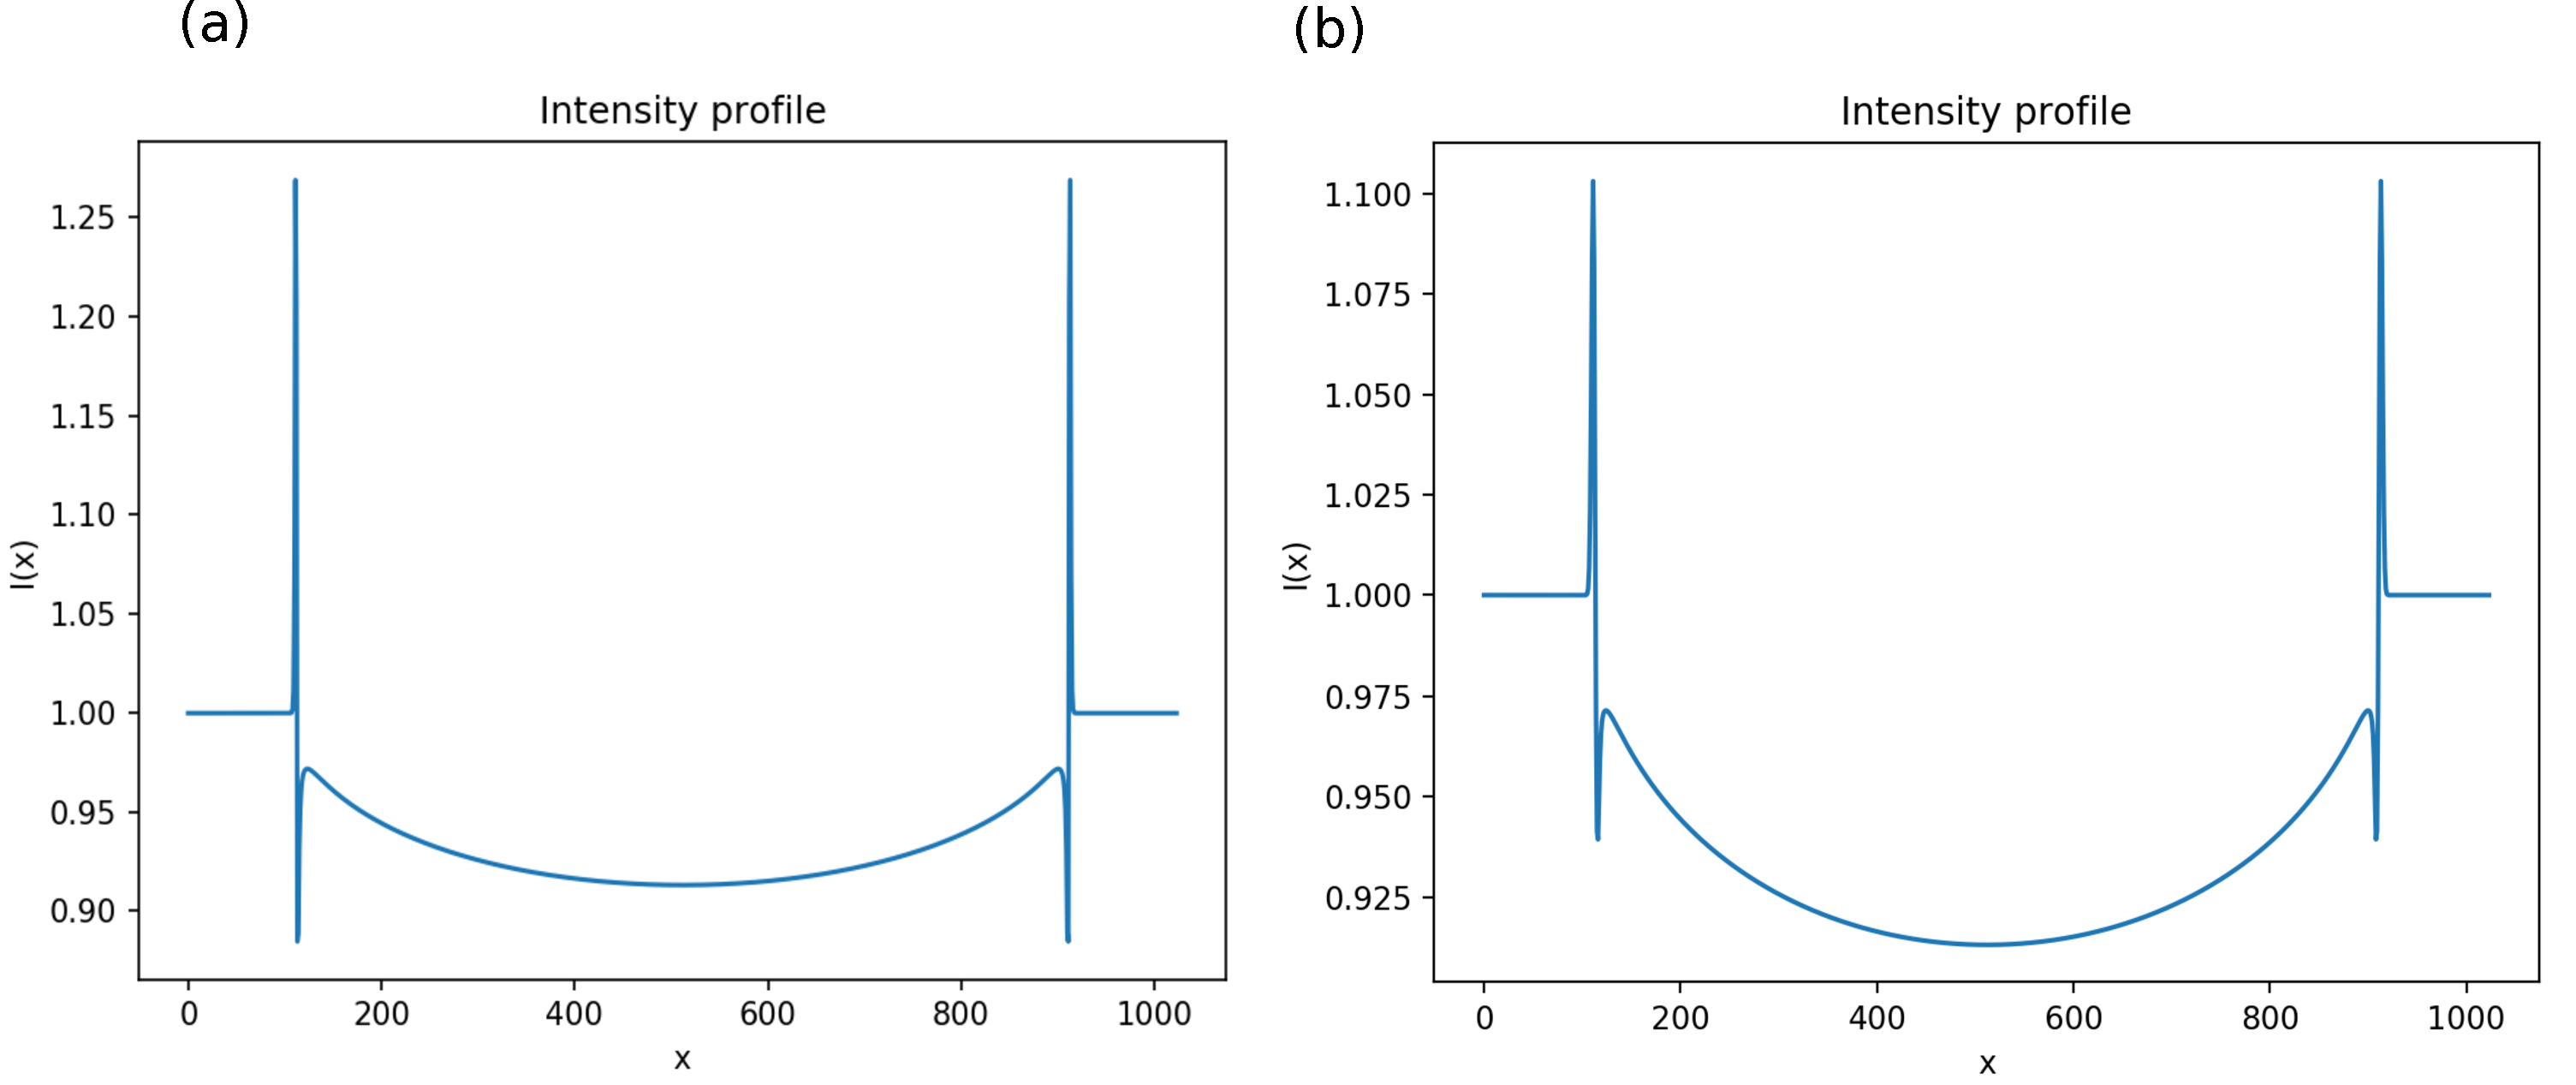
\includegraphics[width=\linewidth]{RK_TEST.pdf}
% \captionof{figure}{Phase contrast cross sections obtained by testing: (a)the finite differences with RK propagation method and (b) the xri TIE. The input parameters and spatial discretisation codes were identical in both (a) and (b). The parameters were for a single cylinder with a radius of  $R = 2$ mm. The X-ray energy used was $50$keV. The refractive index decrement for the water cylinder is $\delta = 9.21425\times 10^{-8}$ and an attenuation coefficient of $\mu = 22.69615\mathrm{m^{-1}}$. In figure (a), the sigmoid function blurred $0.14$ pixels over the edge of the imaged cylinder.  
% The spatial discretisation arrays used in (a) and (b) were both 2D arrays: $x, y = 1024, 1024$ and, the pixel size was $5\mathrm{\mu}$ m. The propagation distance used was $z = 1$ m.}
% \end{Figure}
% \begin{Figure}\label{fig:7}
% \centering
% 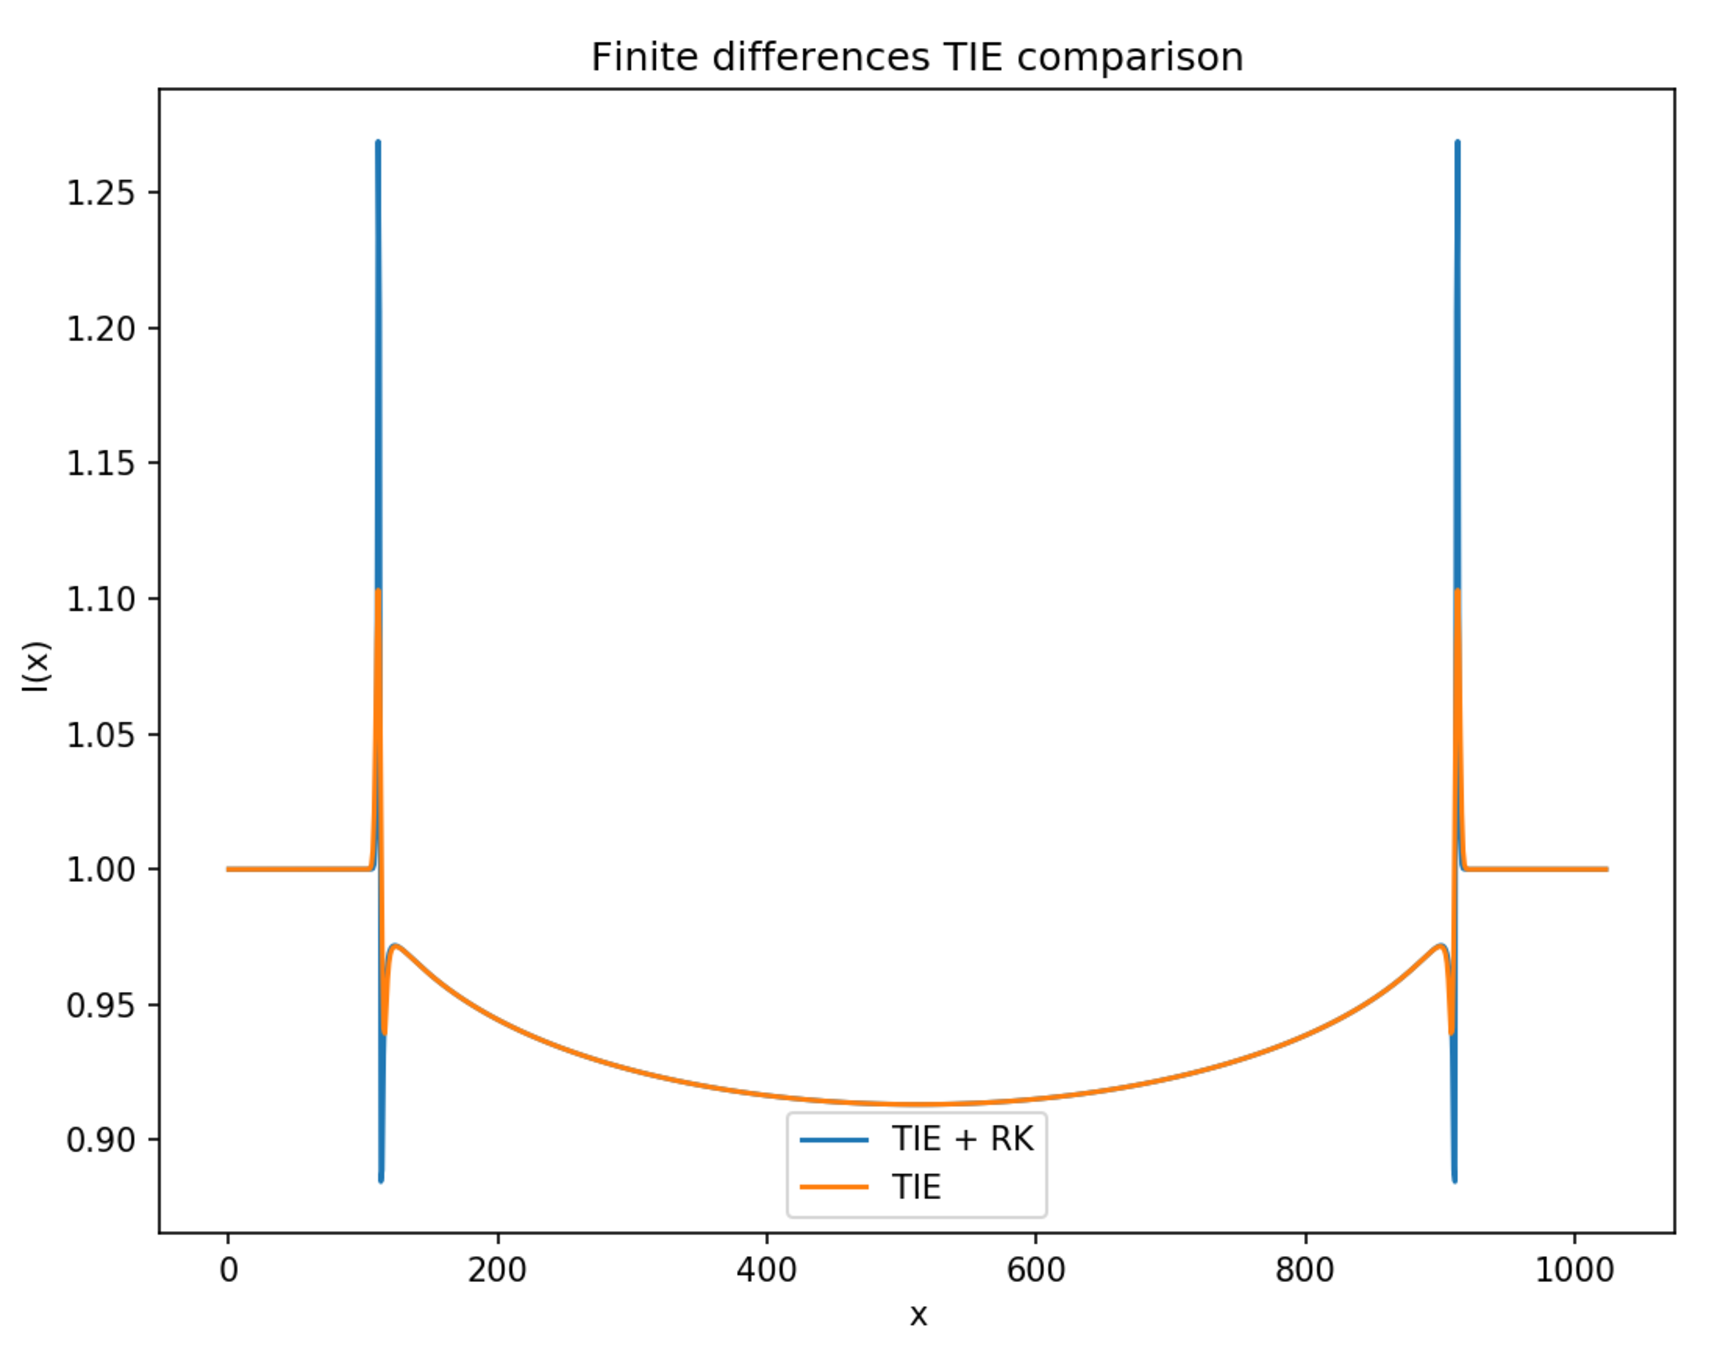
\includegraphics[width=0.6\linewidth]{RK_TEST_difference.pdf}
% \captionof{figure}{Phase contrast cross sections as per figure \ref{fig:6} plotted together to quantify the difference in phase contrast results. The difference in the brightness peaks and troughs between these results are $I_{\mathrm{peak}} = 0.165$ and $I_{\mathrm{trough}} = -0.055$ respectively.}
% \end{Figure}
% The result shown in figures \ref{fig:6} and \ref{fig:7} is interesting because it is possible that the increase in the derivative accuracy from RK could even improve phase retrieval results.

%%%%%%%%%%%%%%%%%%%%%%%%%%%%%%%%%%%%%%%%%%%%%%%%%%%%%%%%%%%%%%%%%%%%%%%%%%%%%%%%%%%%%%%%%%%%%%%%%%%%%%%%%%%%%%%%%%%%%%%%%%%%%%%%%%%%%%%%%%%%%%%%%%%%%%%%%%%%%%%%%%%%%%%%%%%%%
% \section{Future Plans}

% To definitely demonstrate that adding the Runge-Kutta algorithm for spatial propagation drastically improves phase contrast as per figure \ref{fig:5}, I must test my method against other propagation methods used by the X-ray group. These methods include the angular spectrum formulation and Fresnel propagation. If my method consistently yields higher phase contrast, I need to investigate whether higher phase contrast is an accurate measure that would increase the chances of improving phase retrieval results.

% I aim to finish my density simulations by creating a graphic user interface (GUI) that allows the user to modify interactively the density parameters of the imaged concentric cylinders in the simulation. The goal is to make an easily operated visual representation of the changes in phase and intensity of the X-rays as they interact with the imaged object in-situ.

% My supervisor and I are planning to test an X-ray target made of silver which has been obtained for the laboratory apparatus. I need to make simulations using the characteristic radiation spectrum of silver and see how the phase contrast fringes behave when isolating monochromatic X-ray fringes and comparing them to each other. My aim is to eventually obtain real laboratory data and analyse it to compare the efficacy of the new silver target to that of the classic tungsten target currently used in the apparatus.

%%%%%%%%%%%%%%%%%%%%%%%%%%%%%%%%%%%%%%%%%%%%%%%%%%%%%%%%%%%%%%%%%%%%%%%%%%%%%%%%%%%%%%%%%%%%%%%%%%%%%%%%%%%%%%%%%%%%%%%%%%%%%%%%%%%%%%%%%%%%%%%%%%%%%%%%%%%%%%%%%%%%%%%%%%%%%

\chapter{Conclusion}\label{Conclusion}
% In this work I investigate how the phase of incident X-rays changes as the density of distinct sample materials in an arbitrary imaging system changes. I demonstrate that any changes in material density throughout the imaged sample affect the imaging process. I use a _____ 

% simulations to verify if successful phase retrieval can be done of the imaged objects given their variable densities. 


% This report presents a brief outline of the theory behind coherent X-ray imaging, a description of my current progress, and a brief description of my future aims.

%%%%%%%%%%%%%%%%%%%%%%%%%%%%%%%%%%%%%%%%%%%%%%%%%%%%%%%%%%%%%%%%%%%%%%%%%%%%%%%%%%%%%%%%%%%%%%%%%%%%%%%%%%%%%%%%%%%%%%%%%%%%%%%%%%%%%%%%%%%%%%%%%%%%%%%%%%%%%%%%%%%%%%%%%%%%%

\chapter{Acknowledgements}\label{Acknowledgements}

% I want to thank my supervisor Marcus for guiding me through the semester with great suggestions and lots of encouragement. I always enjoyed our talks about physics and other topics. I also want to thank our research group members for being so welcoming and, specifically to Linda for helping me with my writing. Lastly, I want to thank my partner Chris for being an endless source of inspiration, helpful advice and for all our interesting rants and discussions.  

% \begin{center}
% \vspace{5cm}
% \includegraphics[scale=0.2]{bepqed.pdf}
% % \vspace{10cm}
% \end{center}



%%%%%%%%%%%%%%%%%%%%%%%%%%%%%%%%%%%%%%%%%%%%%%%%%%%%%%%%%%%%%%%%%%%%%%%%%%%%%%%%%%%%%%%%%%%%%%%%%%%%%%%%%%%%%%%%%%%%%%%%%%%%%%%%%%%%%%%%%%%%%%%%%%%%%%%%%%%%%%%%%%%%%%%%%%%%%

% %----------------------------------------------------------------------------------------
% %   ABBREVIATIONS
% %----------------------------------------------------------------------------------------

% % \begin{abbreviations}{ll} % Include a list of abbreviations (a table of two columns)

% % \textbf{LAH} & \textbf{L}ist \textbf{A}bbreviations \textbf{H}ere\\
% % \textbf{WSF} & \textbf{W}hat (it) \textbf{S}tands \textbf{F}or\\

% % \end{abbreviations}

\bibliography{mybib}
\bibliographystyle{unsrt}
\end{document}